
\chapter{Results}
\section{Simulation of Capacitance values}
\subsection{Comparision of Capacitance in the simulation with a sphere geometry}
The simulation of the capacitance for the cylindric geometry as a function of different distances with COMSOL leads to the following figure.The simulation of two spheres as well as the approximation formula result in a general 
shift which is due to the fact that it is a three electrode arrangement as the wall of the
low-voltage introduces a new capacitance between the upper electrode and the wall which is not affected by the distance variation. This results in a reduction of the capacitance compared to the 
two spheres geometry. Thus, the simulated values for the low voltage test cell seem reasonable if one compares them to the results of the capacitance between two spheres. \newline 

\begin{figure}[htbp]
	\centering
	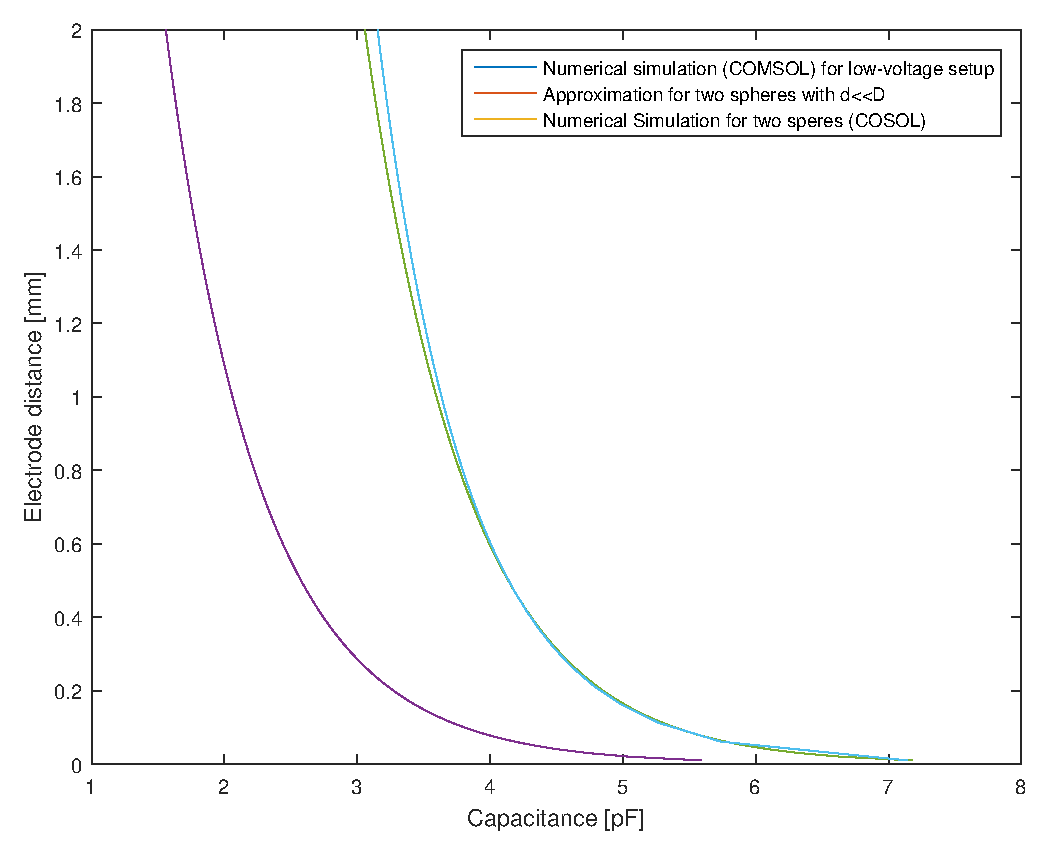
\includegraphics[scale=0.3]{figures/Method/Part1_d_C0/Comparison_Low_voltage_Two_spheres.eps}		
	\caption[Kurze Abbildungsbeschreibung]{Dependency of the electrode distance on the capacitance for the low voltage setup and two spheres $\epsilon = 3.5$ } 
	\label{fig.waveforms}
\end{figure}

\subsection{Complex effective permittivity}
As it was mentioned in the theory chapter, generally speaking, magnitude and phase of the effective permittivity in relation to the
real permittivity of the dielectric are not decoupled quantities. While this effect becomes especially apparent in horizontally layered dielectrics for a
a capacitance with horizontal parallel plates, the graphs below show that the effect for the specimen in the low-voltage cell are negligible. That means a purposely exaggerated variance for both parameters
results in a change in the other parameter that is below 0.1\%.

\begin{figure}[htbp]
	\centering
	\centerline{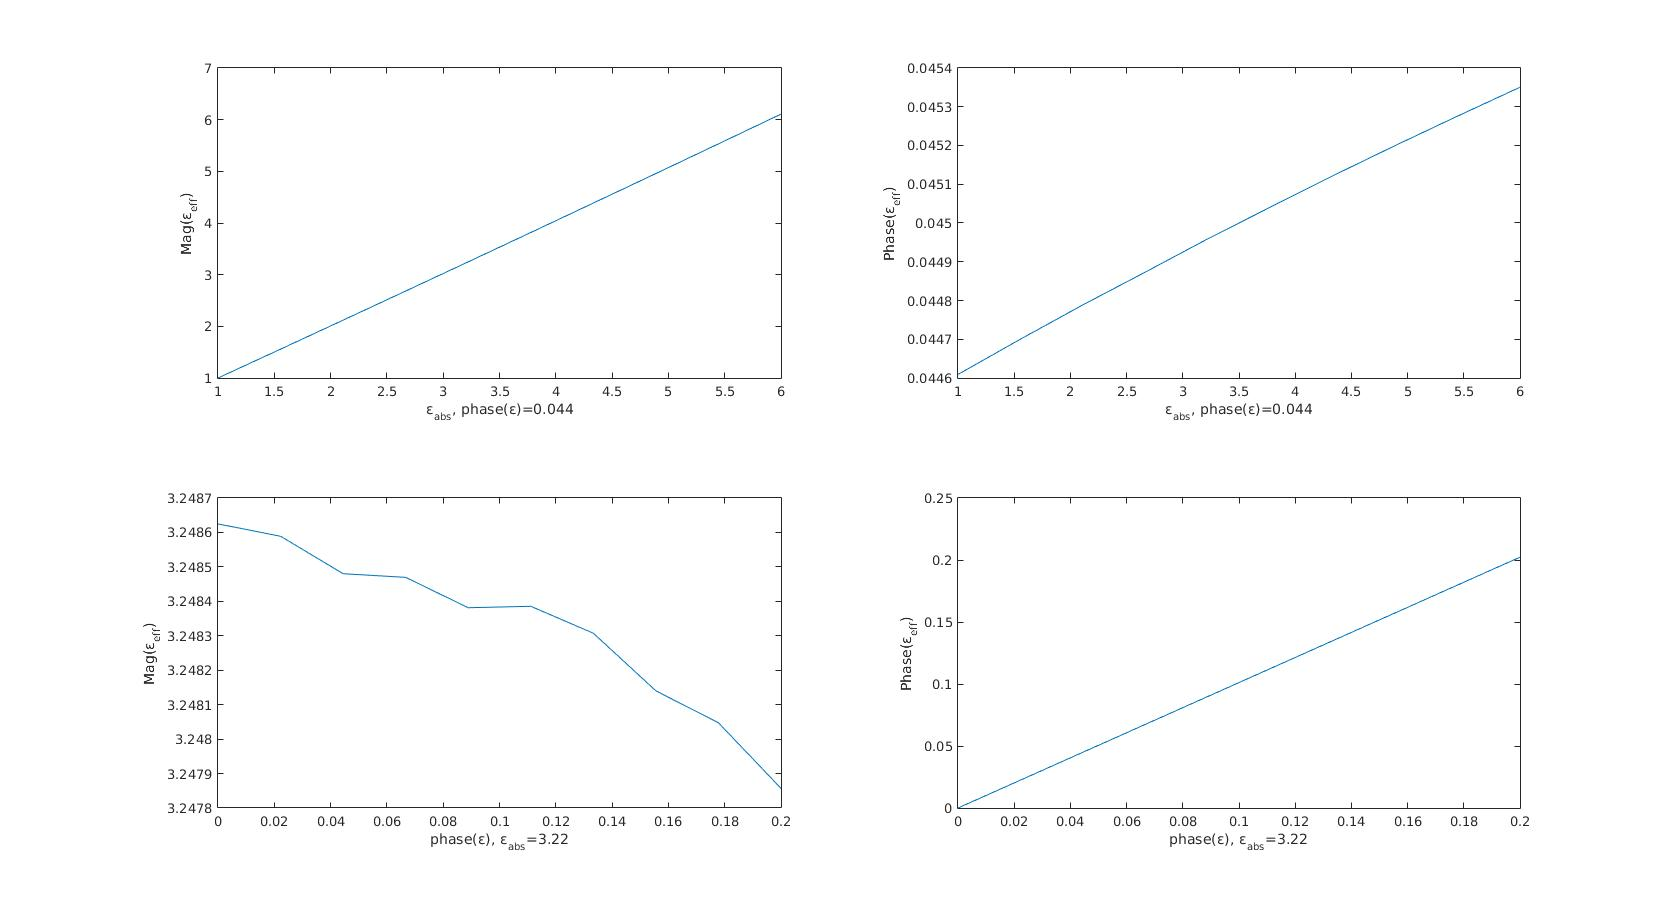
\includegraphics[width=0.5\textwidth]{figures/Results/Complex/complex_permittivity_specimen}}		
	\caption[Kurze Abbildungsbeschreibung]{Interdepedency of phase and magnitude of the effective permittivity (airgap=0.5mm) } 
	\label{fig.complex}
\end{figure}

\section{Capacitance of specimen and effective permittivity}
\begin{figure}[ht]
	\centering
	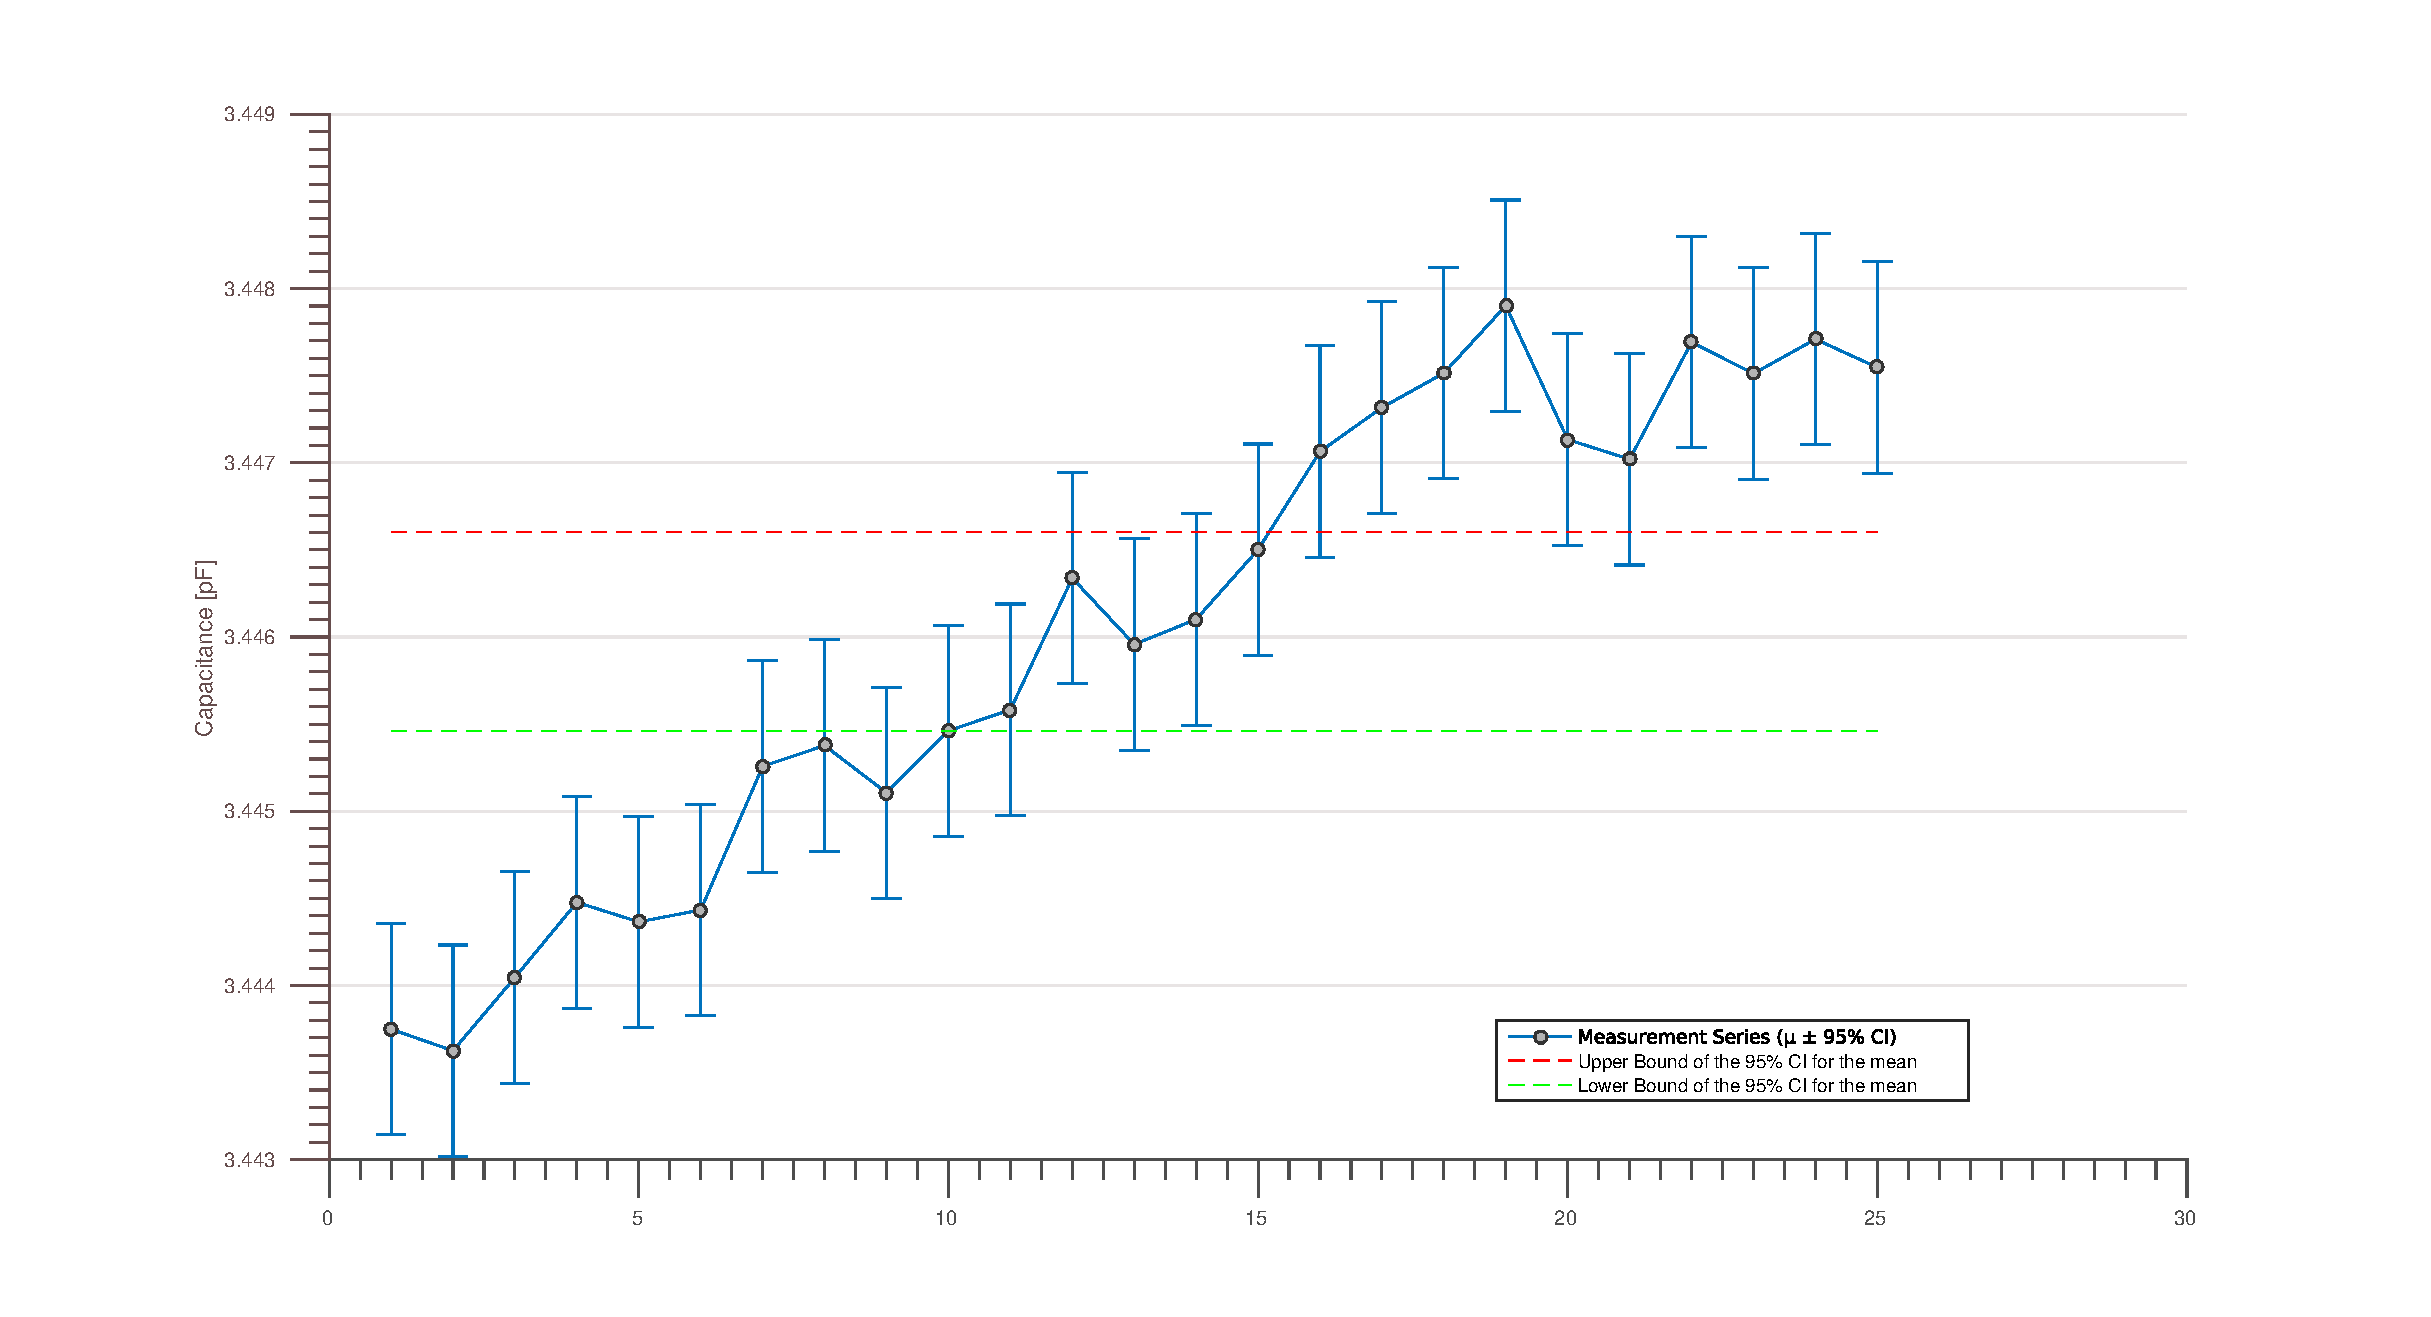
\includegraphics[scale=0.3]{figures/Results/Capacitance_Measure/capacitanceplot.eps}		
	\caption[Kurze Abbildungsbeschreibung]{Measurements of sample capacitance for a series of re-insertions} 
	\label{fig.messreihe}
\end{figure}

The graph \ref{fig.messreihe} effectively contains two measurement series in one. Each one of the gray points represents one measurement in which
the setup was not changed and 25 phase averages were recorded. The resulting confidence interval is depicted by the error bar at each points
and amounts to about 1.12 fF.
\newline
Different gray points were measured by taking out the sample from its container and re-inserting in order to estimate how the results vary in that case.
It turned out that this lead to a much larger measurement variance. Moreover a increase in the capacitance value for each new re-insertion was detected.
And the series of 25 measurements is not enough to predict whether or not if and when the measurements are going to converge, so instead of the maximum difference of
5fF throughout the measurement, a maximum variance of 10fF was assumed.
\newline
For determining the distance, the 
effective dielectric permittivity is assumed to be known. When
considering a maximum electrode distance of 0.25 mm and linearizing the mistake around that point, the 10fF inaccuracy
when measuring the capacitance accounts to about a 11.3 $\mu$m when consulting the look-up table.
The average of the measurements for the magnitude of specimen capacitance amounts to
\begin{equation}
 C_{spec}=3.446pF \pm 5fF
\end{equation}

After the measurement, the same specimen was sawed open in order to perform an optical measurement of the electrode distance.


\begin{figure}[ht]
	\centering
	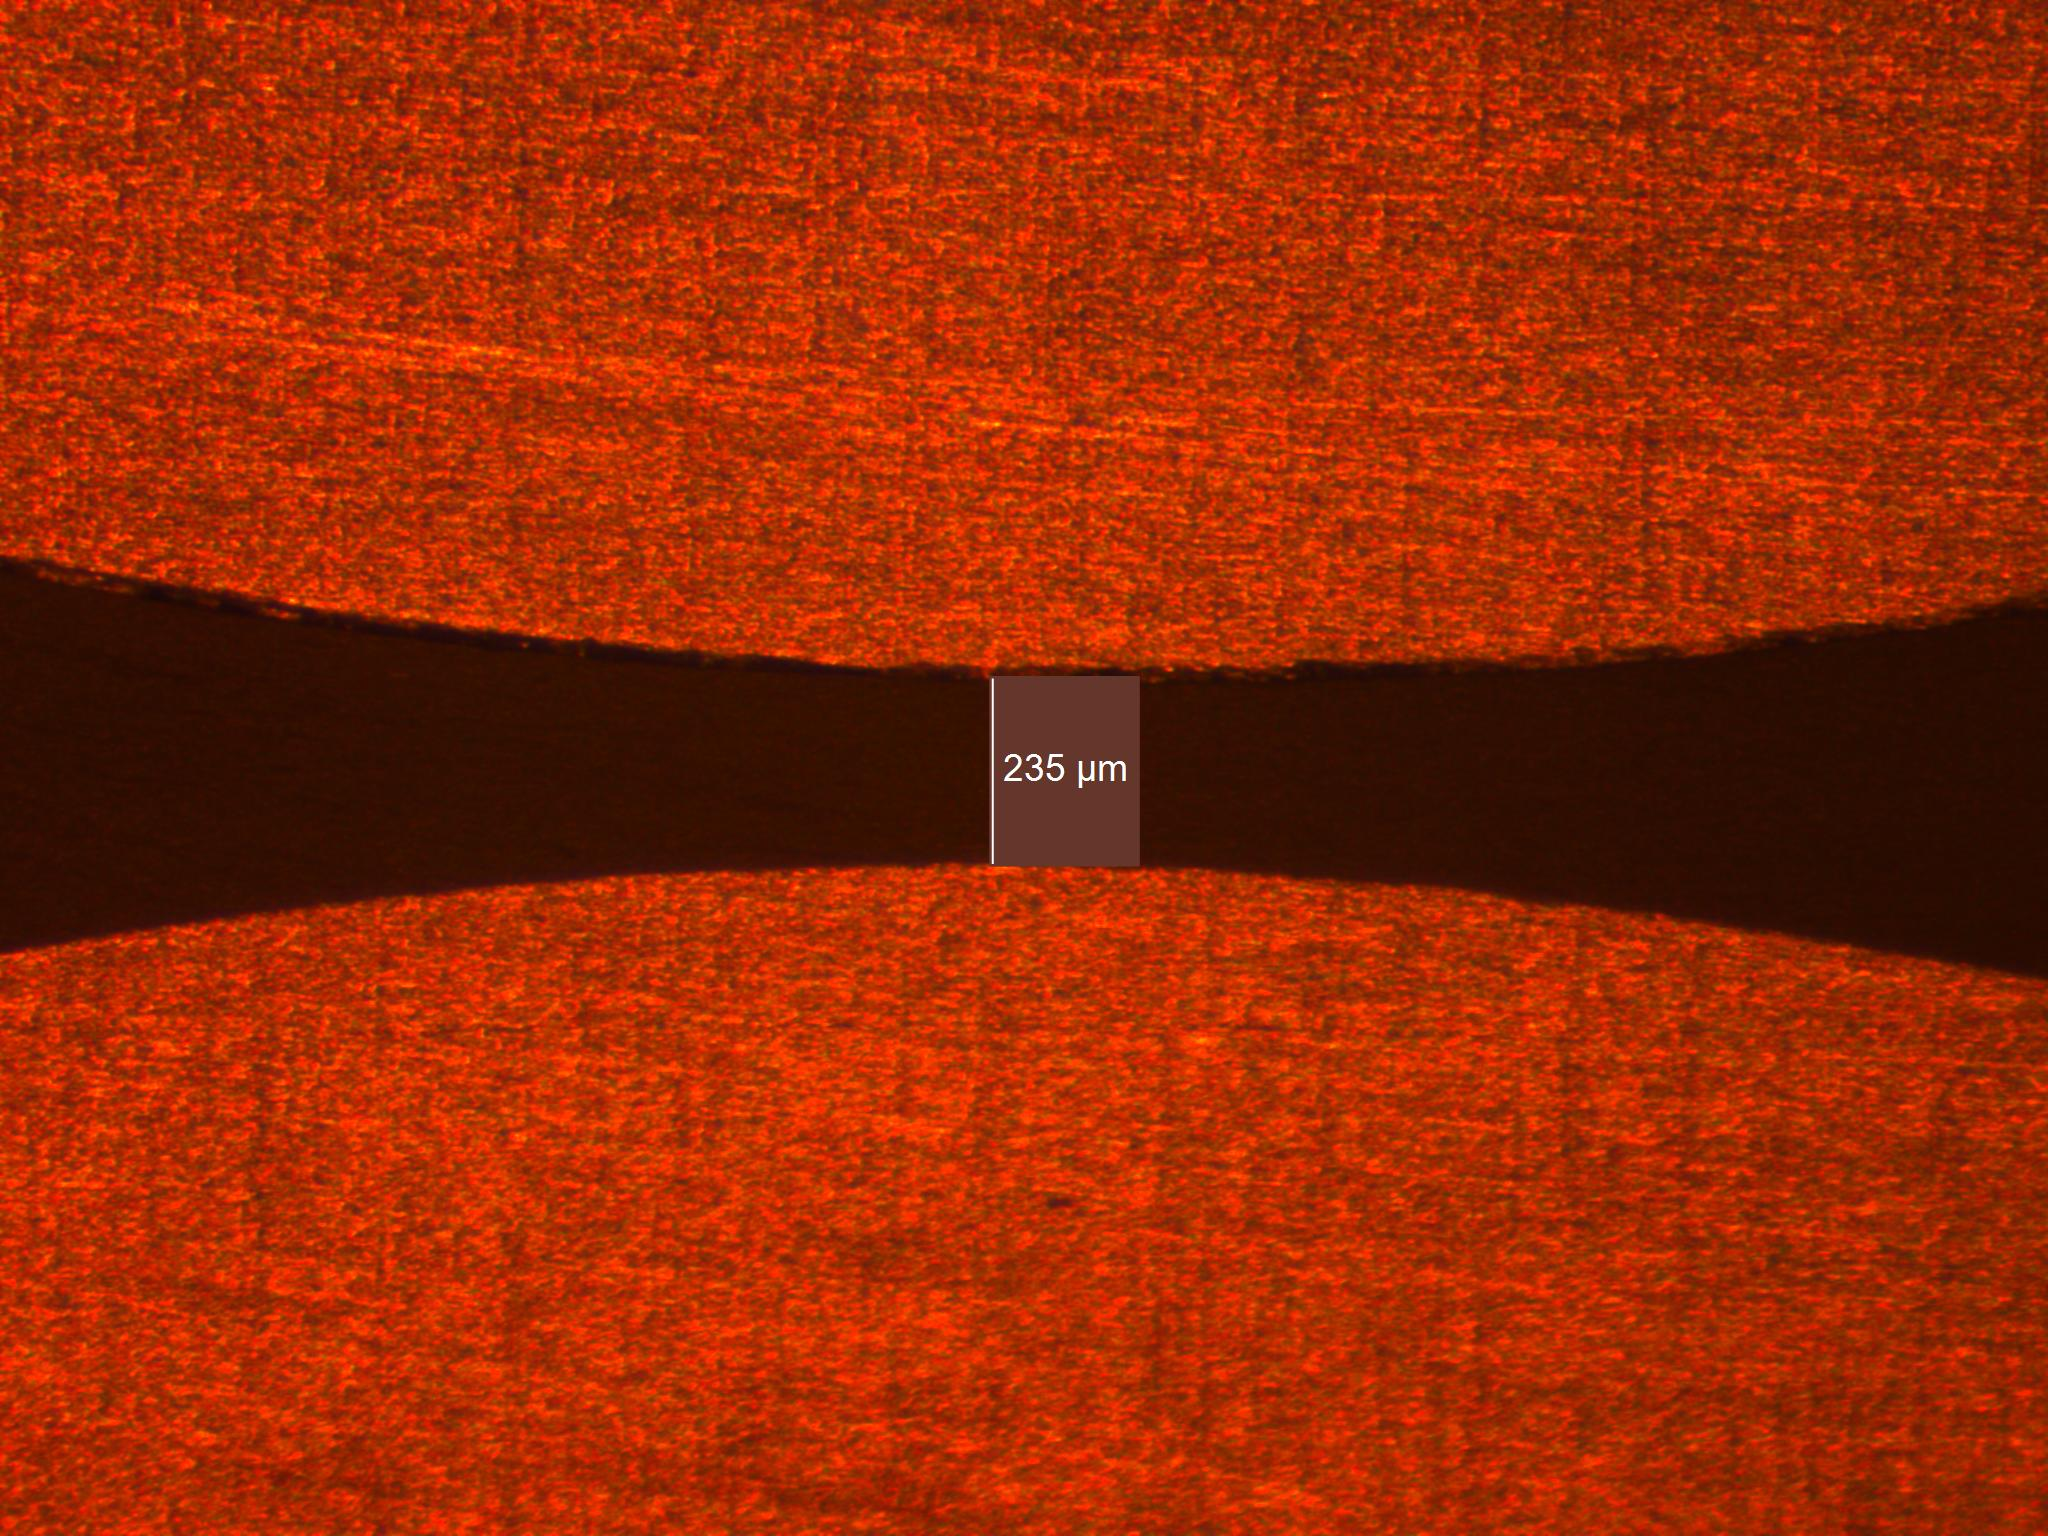
\includegraphics[scale=0.12]{figures/Results/Capacitance_Measure/Sample1_scale.jpg}		
	\caption[Kurze Abbildungsbeschreibung]{Measurements of sample capacitance for a series of re-insertions} 
	\label{fig.opticalmeasurement}
\end{figure}

Using the measured capacitance values in conjunction with the in \ref{fig.opticalmeasurement} determined distance and the look-up table
we find the effective relative permittivity to be:

\begin{equation}
 \epsilon_{eff}=3.85 \pm 0.05
\end{equation}


\section{Current transformer and protective clamping} 
As it was mentioned in the previous chapters, the main advantage to use a current transformer for
dielectric spectroscopy is the fact that the measurement equipment is galvanicaly insulated from the high-voltage supply and its
coupling in case of object breakdown. The analysis of how the current transformer behaves in this case is being conducted in this section.
The peak of the pulses that simulate the breakdown current from the capacitor bank were set to anywhere between 25A and 100A and its duration was about 7 $\mu$s.
The first two experiments were conducted without the protective TVS-Diodes that would limit the ouptut voltage.
The blue curve represents the current through the transformer. The blue line shows how much voltage is applied to a 10 m$\Omega$ shunt resistor and from this information the current can
be deducted. The red line depicts the voltage of the current transformer. To understand the red lines scale, one must consider that firstly, a -40 dB attenuator was placed in front the
oscilloscope and the measurement line was terminated with 50 Ohms, which implies that the real voltage is twice as high as the red curve suggests. For that reason the scale of the red measurement was half the size in order to illustrate the
$\frac{1V}{1A}$ characteristic of the current transformer when taking the blue line as a reference.
\newline 
This leads to the fact that 100mV on the blue scale amount to 10A of current and 10V at the output of the current transformer and the graphs \ref{fig.26Anodiode} to \ref{fig.comparison} should be interpreted
this way.


\begin{figure}[!ht]
	\centering
	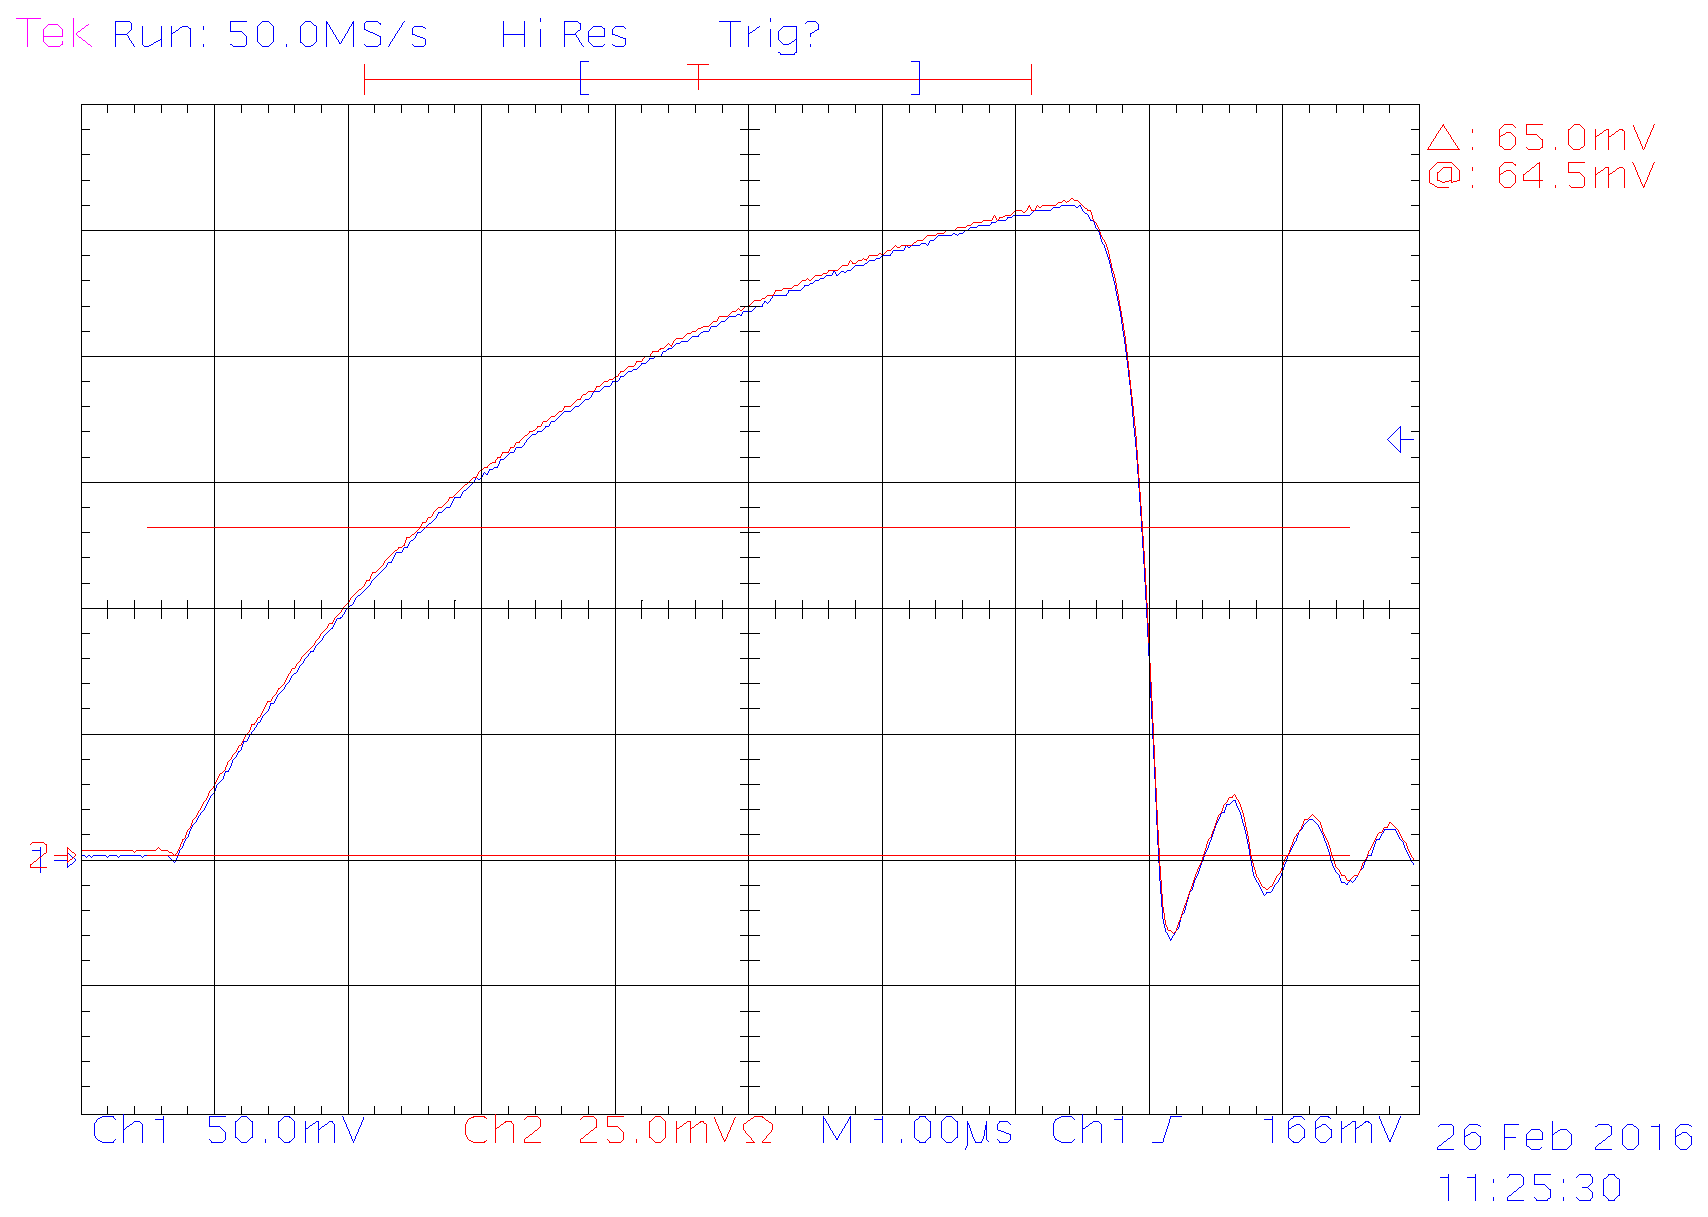
\includegraphics[scale=0.3]{figures/Voltage_Clamping/TEK00001.eps}		
	\caption[Kurze Abbildungsbeschreibung]{26A peak current pulse and no TVS-Diode with resulting voltage} 
	\label{fig.26Anodiode}
\end{figure}

\begin{figure}[!ht]
	\centering
	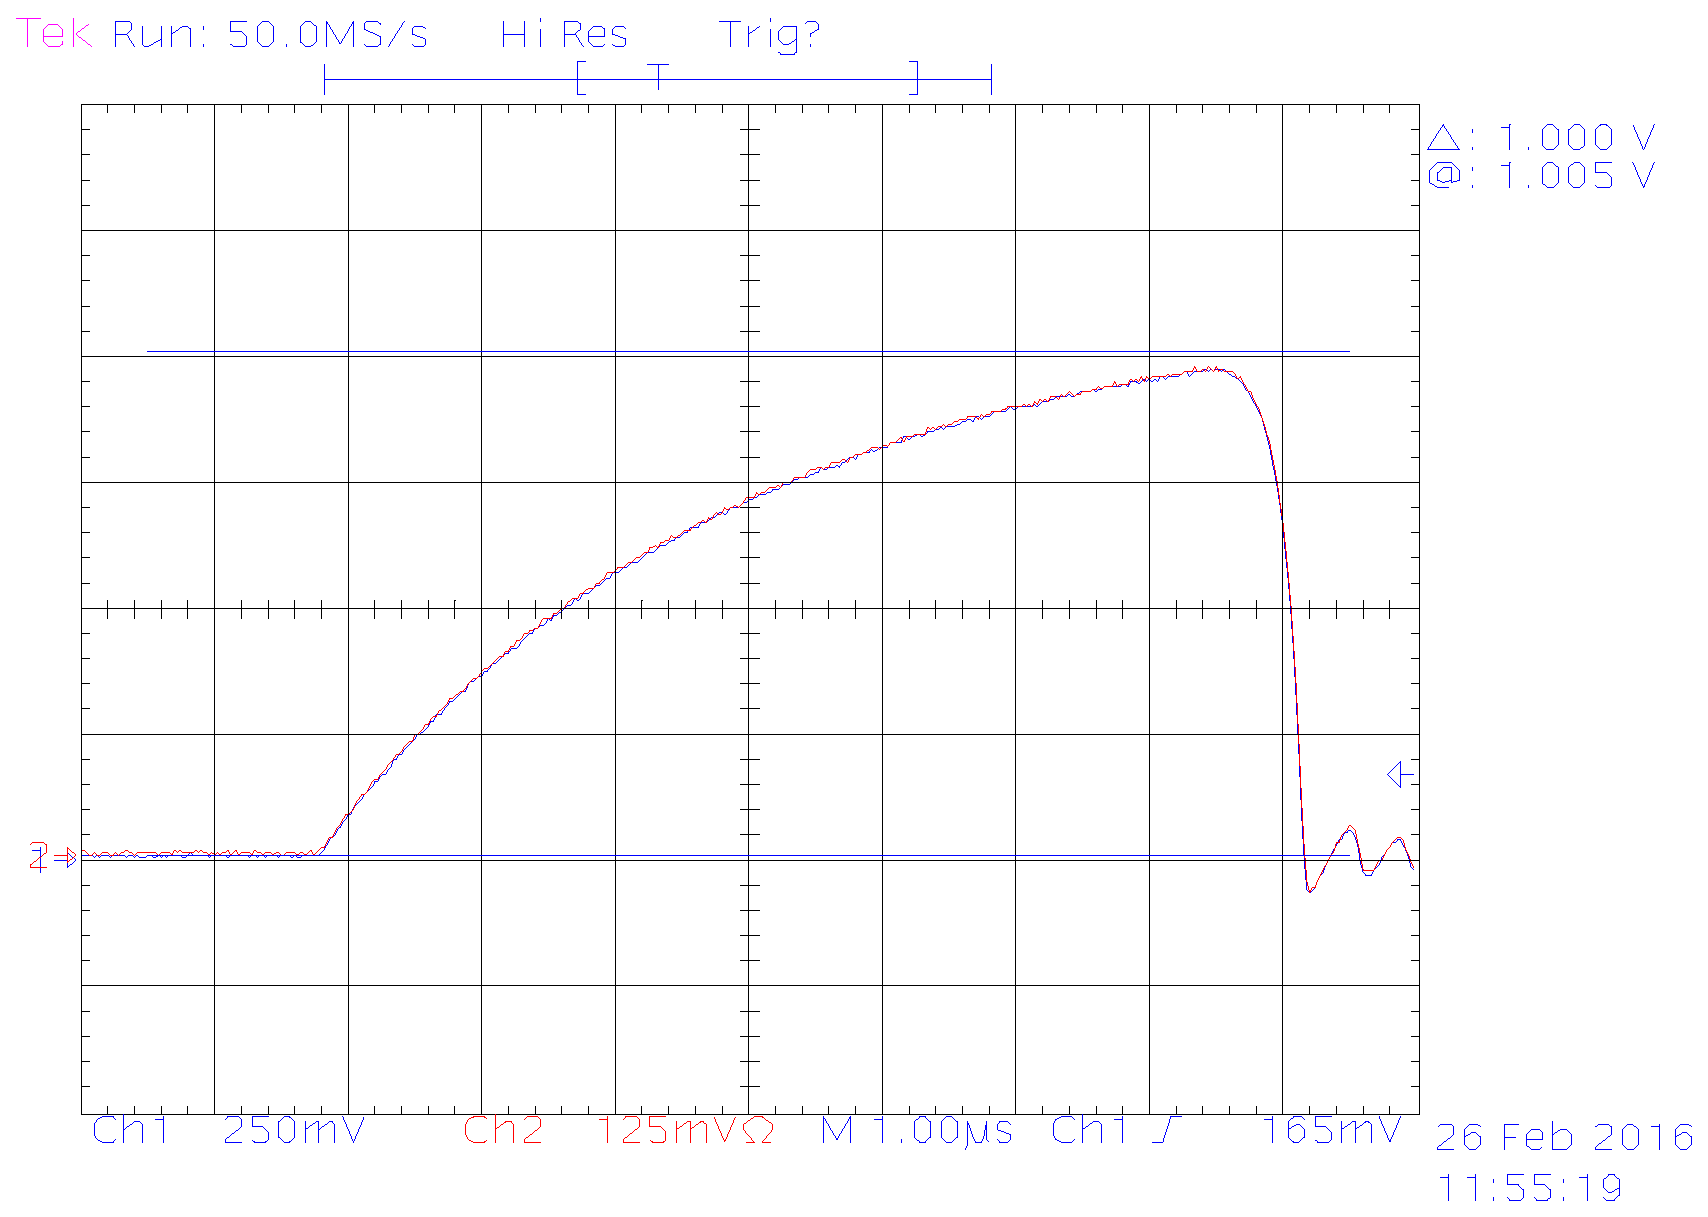
\includegraphics[scale=0.3]{figures/Voltage_Clamping/TEK00004.eps}		
	\caption[Kurze Abbildungsbeschreibung]{95A peak current pulse and no TVS-Diode with resulting voltage} 
	\label{fig.100Anodiode}
\end{figure}

Judging from the graphs \ref{fig.26Anodiode} and \ref{fig.100Anodiode}, the voltage generated by the current transformer aligns almost
perfectly with the current from the capacitor bank.

\begin{figure}[!ht]
	\centering
	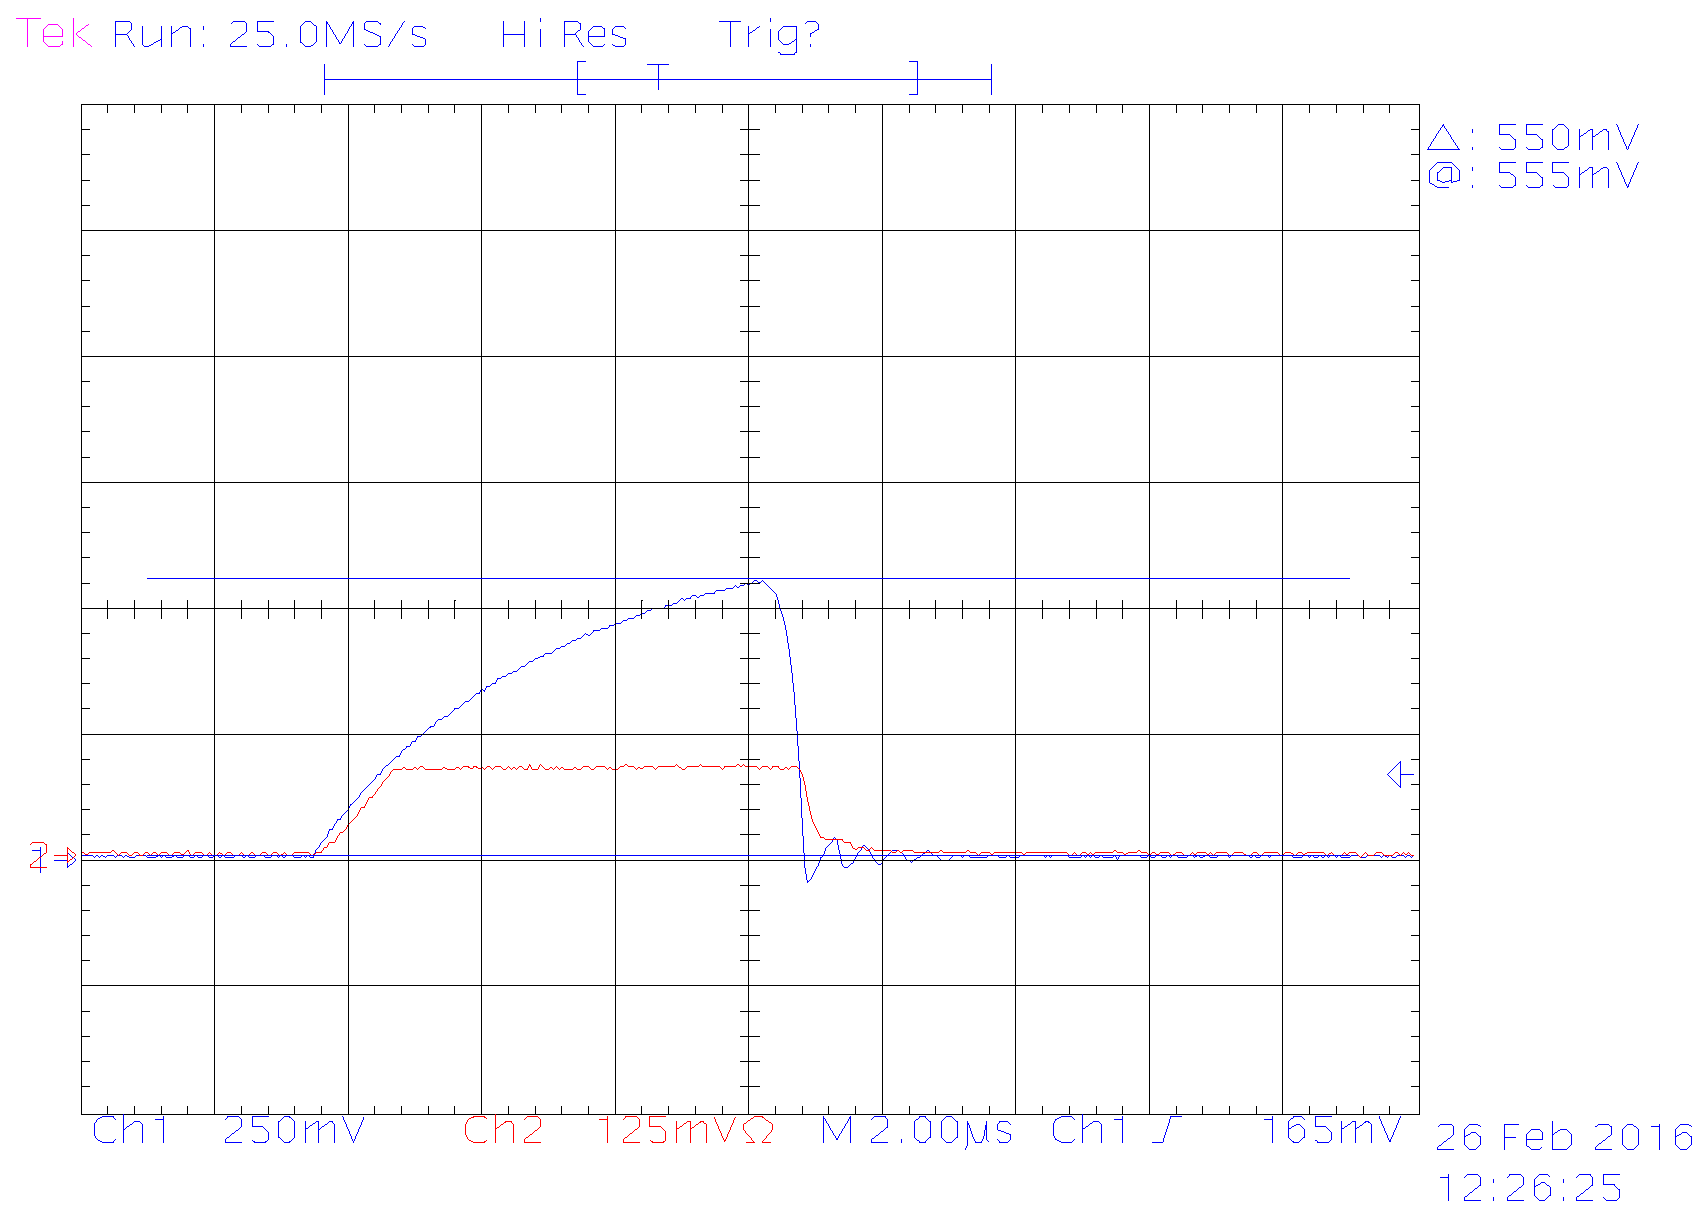
\includegraphics[scale=0.3]{figures/Voltage_Clamping/TEK00006.eps}		
	\caption[Kurze Abbildungsbeschreibung]{53A peak current pulse and inserted TVS-Diode with resulting voltage} 
	\label{fig.53Adiode}
\end{figure}

\begin{figure}[!ht]
	\centering
	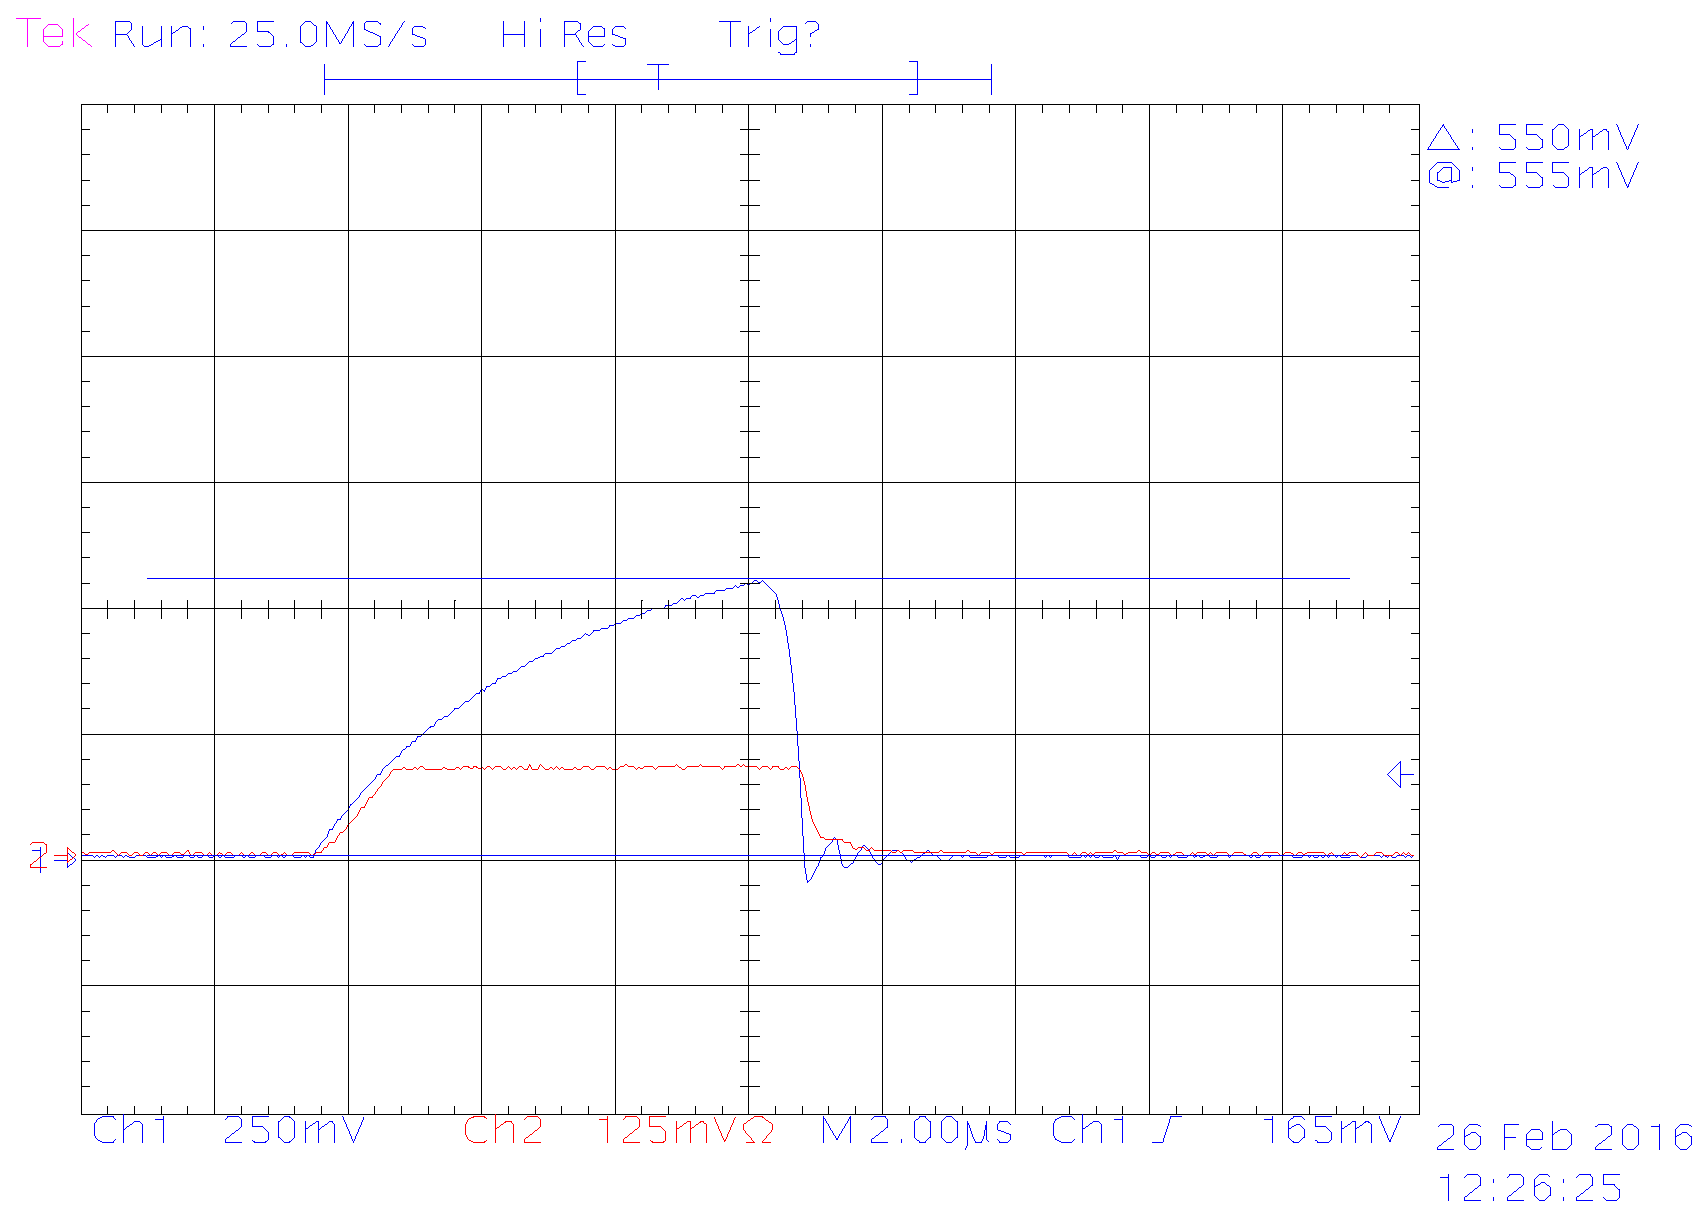
\includegraphics[scale=0.3]{figures/Voltage_Clamping/TEK00006.eps}		
	\caption[Kurze Abbildungsbeschreibung]{102A peak current pulse and inserted TVS-Diode with resulting voltage} 
	\label{fig.100Adiode}
\end{figure}

The recorded current and voltage from \ref{fig.53Adiode} and \ref{fig.100Adiode} show on
one hand that the protective diodes reliably clamp the voltage once it would normally go above 17.5 V even
independent of how high the actual current throught the current tranformer is. But on the other hand, the signals are no longer as similar as they were 
without the clamping.


This fact becomes even more apparent when we analyze currents that do not result in a voltage above the clamping voltage.
In figure it can be noticed how the red curve struggles to follow the current and even in the oscillation part at the end a remarkable phase shift was detected which results in a significant
mistake.


\begin{figure}[ht]
	\centering
	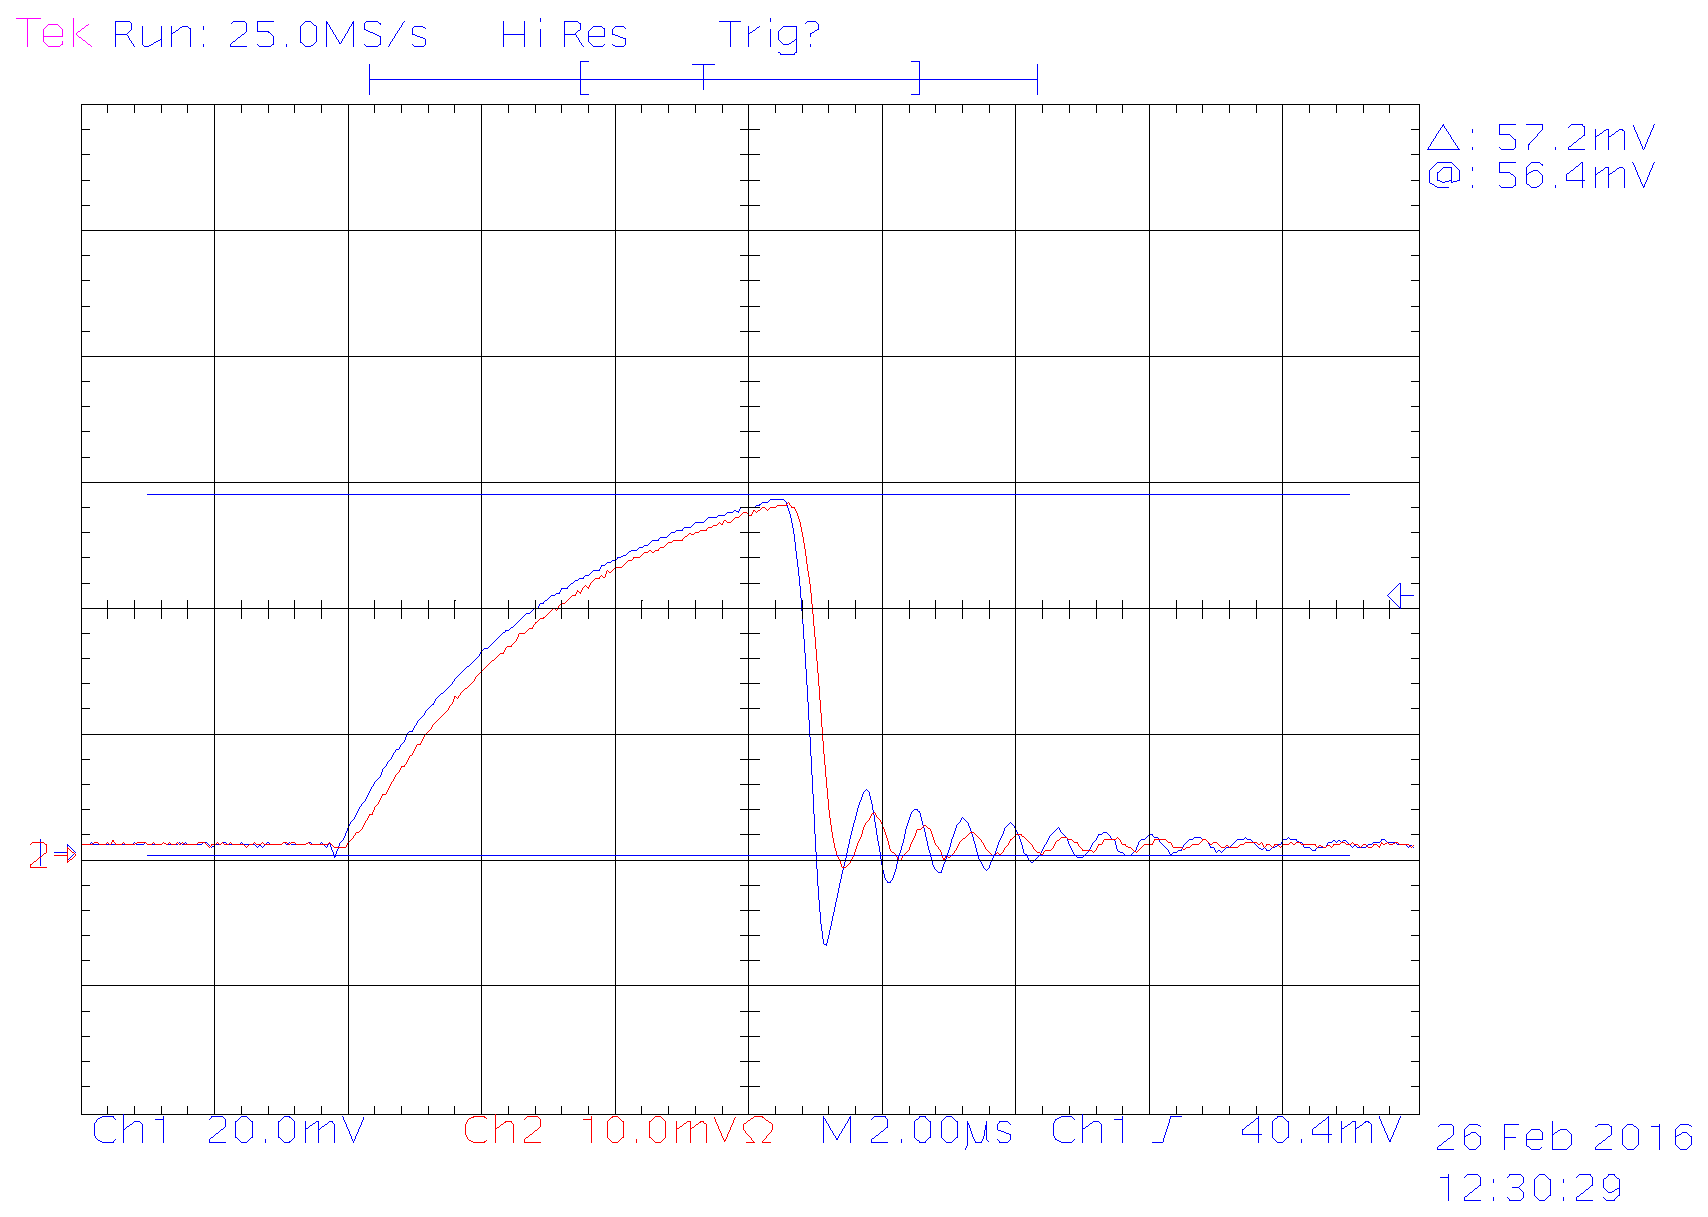
\includegraphics[scale=0.3]{figures/Voltage_Clamping/TEK00008.eps}		
	\caption[Kurze Abbildungsbeschreibung]{5.8A peak current pulse and inserted TVS-Diode with resulting voltage (no clamping)} 
	\label{fig.comparison}
\end{figure}

\section{Dielectric Spectroscopy}
\subsection{Loss tangent}
\begin{figure}[htbp]
  \centering
  \centerline{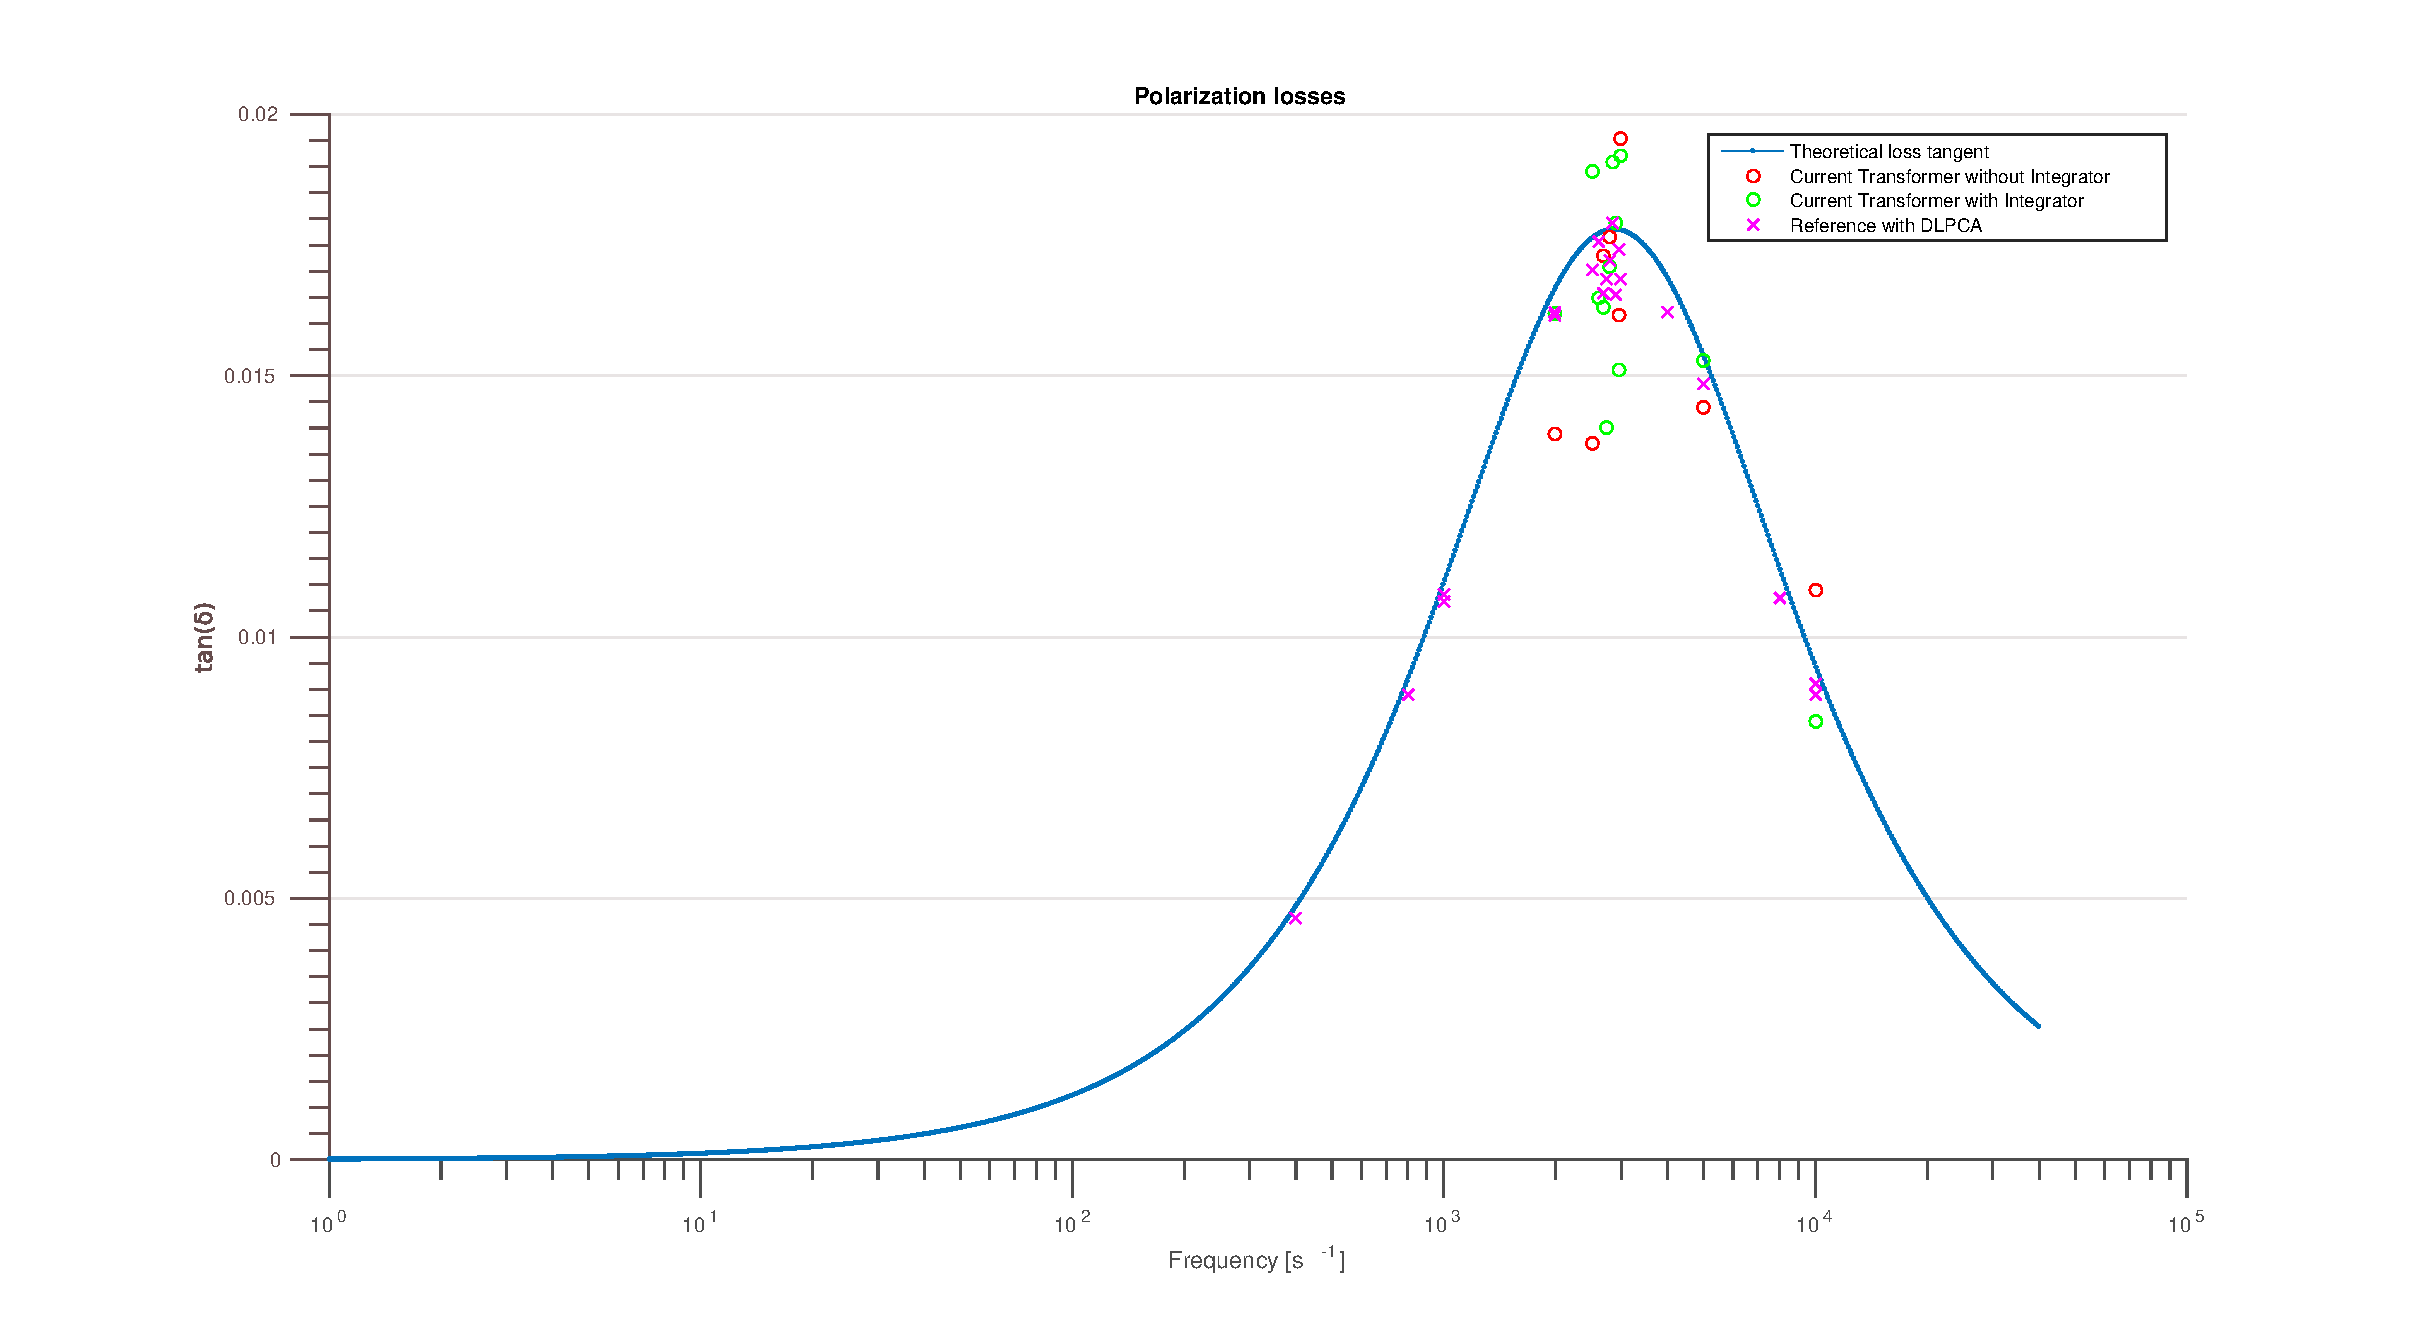
\includegraphics[scale=0.3]{figures/Results/Spectroscopy/spectroscopywithoutbars}}
  \caption[Kurze Abbildungsbeschreibung]{Measurements of dielectric loss tangent in different setup configurations}

  \label{fig.spectroscopy}

\end{figure}
The three data series created from the spectroscopy experiment using the Debye model are shown in the graph above. The solid blue line represents the theoretical  dielectric loss tangent given the parameters of the components in the debye model
as a function of the frequency.
The components were assumed to be ideal and not to be temperature dependent.
The magenta data points can be used as a reference to evaluate the performance of the current transformer as these measurement points
were obtained with a industry standard low-noise current amplifier (DLPCA). 
The red points were recieved by replacing the DLPCA with the current transformer.
The green points were measured with the integrator in place, effectively integrating the voltage signal generated by the current transformer.

\begin{figure}[htbp]
 \centering
 \centerline{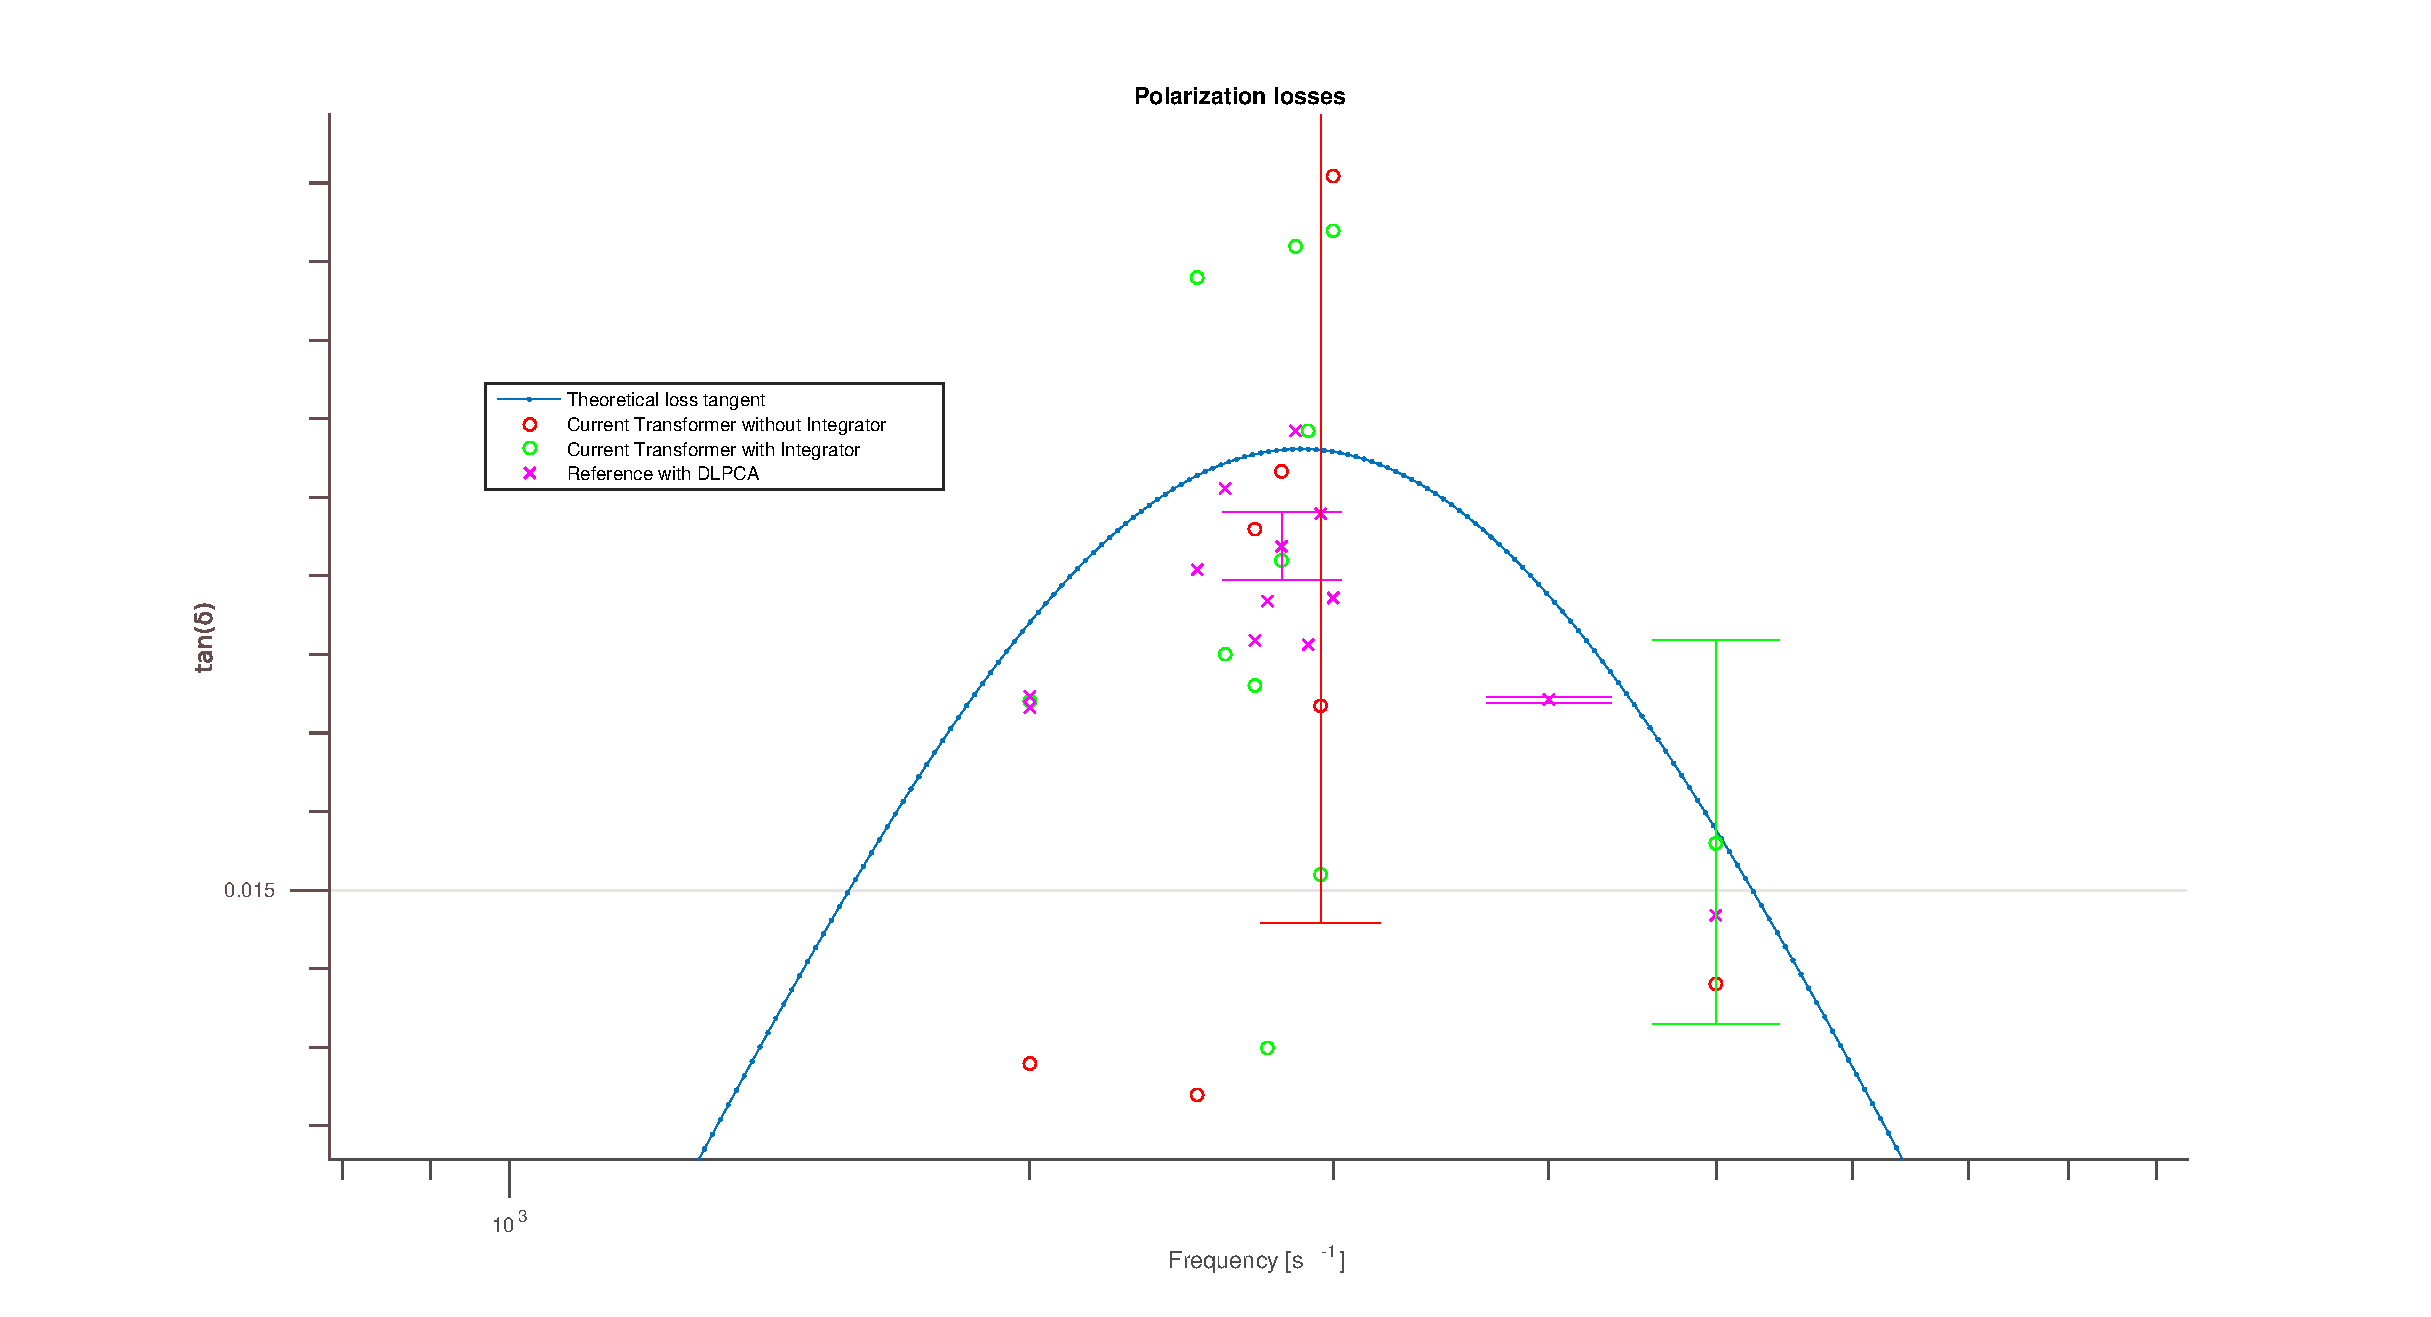
\includegraphics[scale=0.3]{figures/Results/Spectroscopy/errorbarsbettercolor}}

\caption[Kurze Abbildungsbeschreibung]{Confidence intervals}
\label{fig.spectroscopy2}
\end{figure}

In order to adequately analyze the data points, the above graphic shows the previous plot
zoomed in around the maximum loss tangent since the deviation from the theoretical result seem to be the largest here.
The confidence intervals were added for a few points in each measurement series.

First it can be noted that while the reference measurements fit the curve the closest, the theoretical values are still not
within the measurements confidence intervals and the error can be greater than 10\%. To sum up the measurements conducted with
the current transformer, it can be stated that the measurement performance was significantly worse than the reference. Not only do they deviate further from the theoretical values
but they also have a larger variance. Which means that one cannot consistently predict a reasonable range for the mean of said measurement, at least not for only 9 phase averages.
While the use of the integrator succesfully lowered the deviation and shrinked the confidence intervals by a factor of 2 to 3, the measurement accuracy is still nowhere close to the one obtained with the DLPCA.

\subsection{Analysis of Noise Parameters}

In order to identify one of the sources to which the errors can be attributed, the noise level at the input and at the ouput was measured and analyzed to gain an estimation about how much noise was added in the system.
Using the current transformer in both configurations, i.e. with and without the integrator, the following parameters were measured. They will be put in perspective when comparing them to the first table that includes the same quantites for the DLPCA setup.


\textit{Data for the DLPCA:}


\begin{center}
\begin{tabular}{|m{3cm}|m{3cm}|m{2.5cm}|m{3.2cm}|m{2cm}|} 
\hline
frequency [Hz]& SNR$_{in}$ & SNR$_{out}$ & Noise Figure [dB] & Noise Floor \\ 
\hline \hline
2000 &  8.25E+06 &  3.74E+05 & 13.43 & 1.00E-05 \\ 
\hline
2500 & 6.95E+06 & 6.02E+05 & 10.62 & 1.00E-05 \\ 
\hline
2700 & 3.92E+05 & 2.19E+05 & 2.53 & 1.00E-05 \\ 
\hline
3000 & 6.5E+04 & 4.72E+04 & 1.39 & 1.00E-05 \\ 
\hline
5000 & 2.331E+06 & 4.40E+06 & 2.76 & 1.00E-05 \\ 
\hline
\end{tabular}
\end{center}


\textit{Data without integrator:}
\begin{center}
\begin{tabular}{|m{3cm}|m{3cm}|m{2.5cm}|m{3.2cm}|m{2cm}|} 
\hline
frequency [Hz]& SNR$_{in}$ & SNR$_{out}$ & Noise Figure [dB] & Noise Floor \\ 
\hline \hline
2000 & 2.40E+07 & 16.31 & \cellcolor{blue!25}61.79 & 1.00E-05 \\ 
\hline
2500 & 1.8E+07 & 25.69 & \cellcolor{blue!25}58.55 & 1.00E-05 \\ 
\hline
2700 & 5.10E+07 & 31.02 & \cellcolor{blue!25}42.23 & 1.00E-05 \\ 
\hline
3000 & 5.13E+05 & 42.04 & \cellcolor{blue!25}40.86 & 1.00E-05 \\ 
\hline
5000 & 7.17E+06 & 79.386 & \cellcolor{blue!25}49.56 & 1.00E-05 \\ 
\hline
10000 & 1.09E+06 & 377.35 & \cellcolor{red!25}34.616 & 1.00E-04 \\ 
\hline

\end{tabular}
\end{center}

\textit{Data with integrator:}
\begin{center}
\begin{tabular}{|m{3cm}|m{3cm}|m{2.5cm}|m{3.2cm}|m{2cm}|} 
\hline
frequency [Hz]& SNR$_{in}$ & SNR$_{out}$ & Noise Figure [dB] & Noise Floor \\ 
\hline \hline
2000 & 3.00E+07 & 35.23 & \cellcolor{blue!25}59.35 & 1.00E-05 \\ 
\hline
2500 & 1.77E+07 & 78.12 & \cellcolor{blue!25}53.5 & 1.00E-05 \\ 
\hline
2700 & 3.60E+05 & 39.05 & \cellcolor{blue!25}40.6 & 1.00E-05 \\ 
\hline
3000 & 3.17E+05 & 113.1 & \cellcolor{blue!25}34.47 & 1.00E-05 \\ 
\hline
5000 & 8.90E+06 & 23.44 & \cellcolor{blue!25}41.7 & 1.00E-05 \\ 
\hline
10000 & 1.10E+06 & 22.5 & \cellcolor{red!25}46.9 & 1.00E-04 \\ 
\hline

\end{tabular}

\end{center}
When a sinusoidal input is applied to the system. The SNR was defined as the ratio of the energy in the FFT-bin that corresponds
to the fundamental frequency of the oscillation and the energy of all other components. Since the distance of the sampling in the time domain was chosen
such that the first index shows the proportion of the fundamental frequency in the signal, the signal to
noise ratio can be defined as follows.


\begin{equation}
SNR=\frac{\hat{x}[1]^2}{\sum\limits_{i=0,i\neq1}^{N}\hat{x}[i]^2}
\end{equation}

The noise figure relates the noise level at the input and the output and therefore is a measure of the added noise of the measurement setup:

\begin{equation}
 Noise\,Figure\, [dB]=10log\left(\frac{SNR_{in}}{SNR_{out}}\right)
\end{equation}

Noise floor is a parameter that declares around which value the spectral components of the higher frequencies, i.e. noise are located. Generally it can be said that the higher the noise floor is,
the higher the variance in the measurement of the dielectricl loss tangent.\cite{FaerberMVISS}
When using the current transformer, it has to be taken into account that between the frequencies of 2000 Hz up to 5000 Hz, a degradation of the noise
figure of about 40-50 dB has to be expected. However one must consider that the DLPCA used a variable gain in order to generate an output whose amplitude amounts to about 10V which takes advantage of the full resolution of the 
digital to analog converter, whereas in the other two setups the gain was set to a constant value.
The noise figure does in fact decrease when the integrator is in use. Yet, most likely due to the non-idealities described in the next section, the noise figure varied within 5dB for the same frequency. 
The calculated values for the noise figure for the setup with integrator were still consistently lower than the one for the setup without it for frequencies up to 5000 Hz.

The following figures illustrate the spectral distribution of the noise for 2000 Hz at the output for a sinusoidal input. Using these graphs, the above mentioned value for the noise floor can be determined.


\begin{figure}[htbp]
 \centering
 \centerline{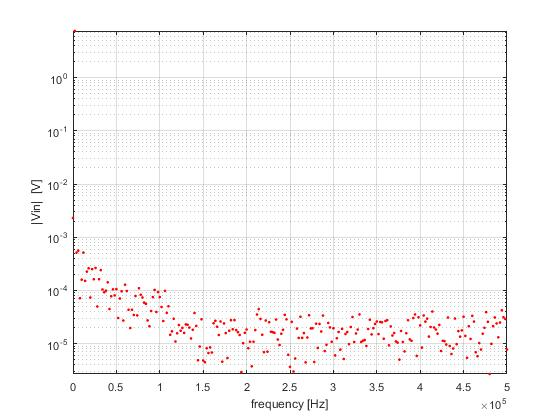
\includegraphics[scale=0.3]{figures/Results/NoiseFloor/DLPCA.jpg}}

\caption[Kurze Abbildungsbeschreibung]{Noise Floor of Measurement with DLPCA }
\label{fig.noisefloordlpca}
\end{figure}

\begin{figure}[htbp]
 \centering
 \centerline{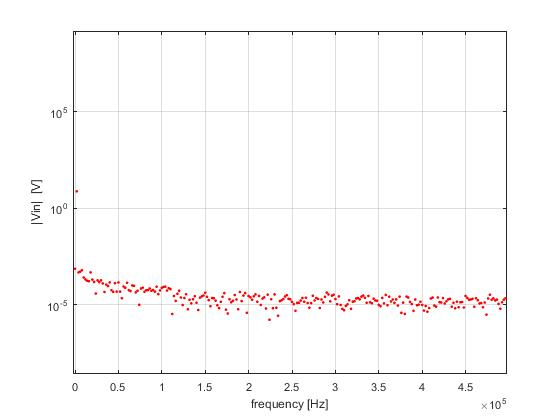
\includegraphics[scale=0.3]{figures/Results/NoiseFloor/currenttransformer.jpg}}

\caption[Kurze Abbildungsbeschreibung]{Noise Floor of Measurement with current transformer }
\label{fig.noisefloorcurrentt}
\end{figure}

\begin{figure}[htbp]
 \centering
 \centerline{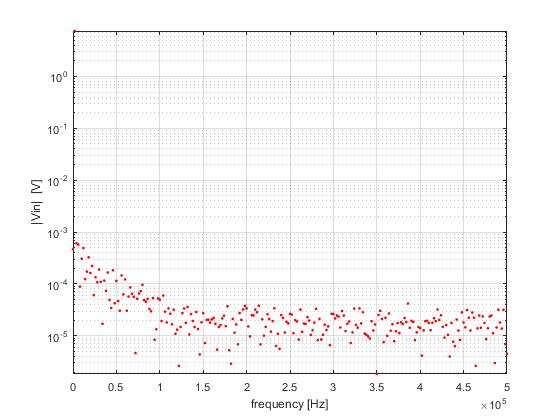
\includegraphics[scale=0.3]{figures/Results/NoiseFloor/Integrator.jpg}}

\caption[Kurze Abbildungsbeschreibung]{Noise Floor of Measurement with current transformer and integrator }
\label{fig.noisefloorintegrator}
\end{figure}




\section{Performance of integrator}
As described in the previous two passages, the integrator was capable of reducing the noise figure and hence effectively reducing 
the confidence interval when determining the dielectric loss tangent. While measuring the output of the integrator, particularily two unexpected problems were determined.
First, a DC offset at the output, that was varying with different input signals was detected. For an applied voltage, that had the shape of the expected transformed current pulse train
flowing through the debye equivalent, this offset could not be eliminated by tuning the potentiometer at the operational amplifier.

\begin{figure}[htbp]
 \centering
 \centerline{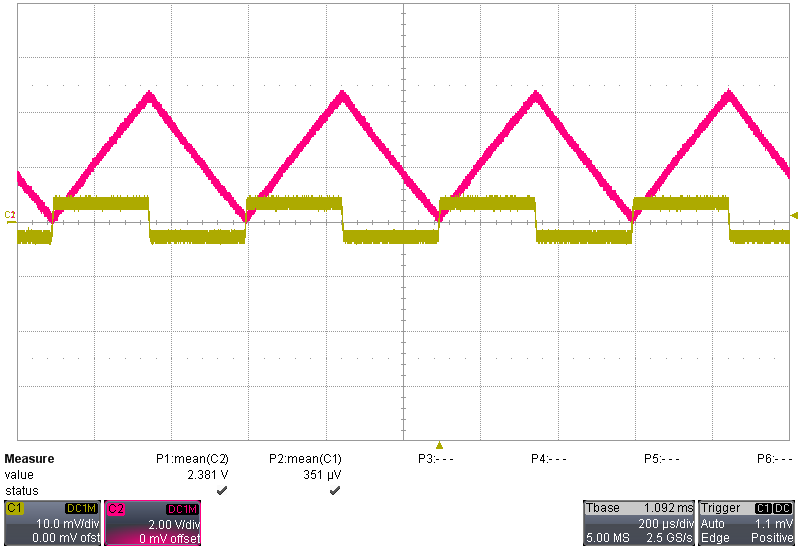
\includegraphics[scale=0.3]{figures/Results/Integrator_measurements/voltwave_10us}}

  \caption[Kurze Abbildungsbeschreibung]{Output in magenta applying a rectangular voltage signal with a rise time of 10 microseconds at the input}
\label{fig.voltwave_10us}
\end{figure}

Secondly, even when the same periodic signal was applied at the input of the integrator, a low frequency oscillation was imposed onto the output signal.
\begin{figure}[htbp]
 \centering
 \begin{minipage}{0.4\textwidth}
 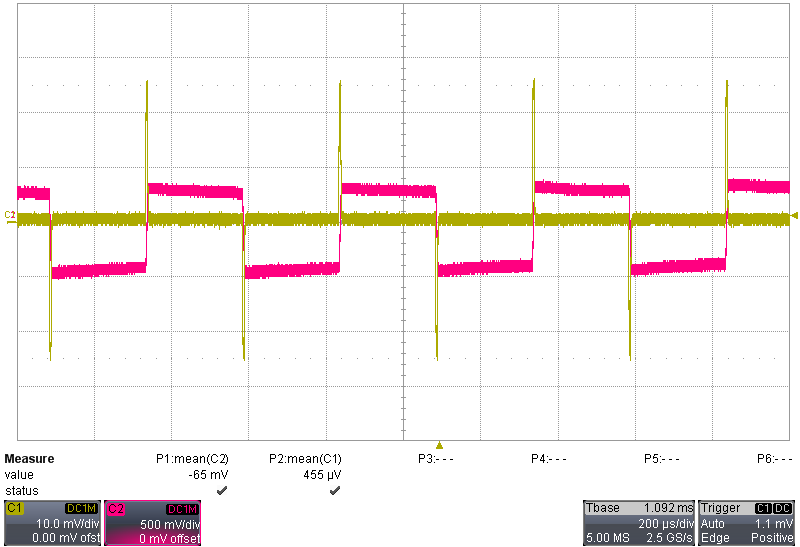
\includegraphics[scale=0.2]{figures/Results/Integrator_measurements/currentwave_10u}
 \caption[Kurze Abbildungsbeschreibung]{Applying the current pulse caused by a rectangular voltage signal with a rise time of 10 microseconds at one instant. }
 \end{minipage}\qquad
 \begin{minipage}{0.4\textwidth}
 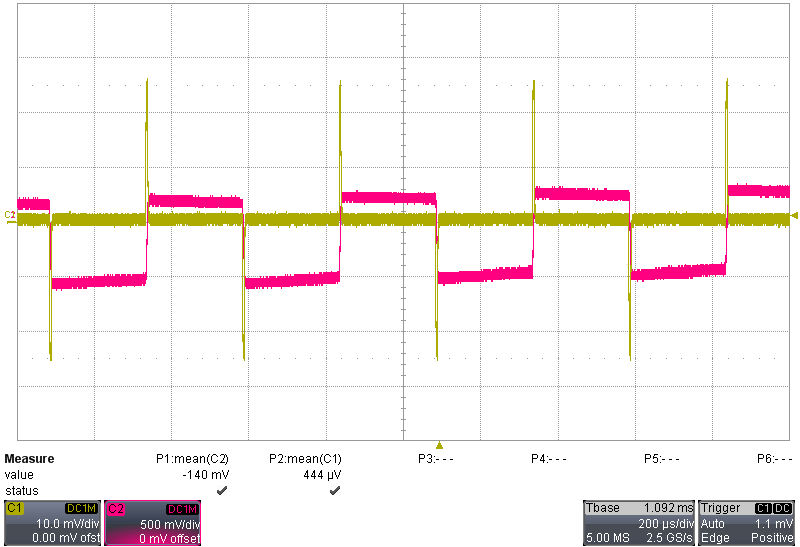
\includegraphics[scale=0.2]{figures/Results/Integrator_measurements/cuwave_10u-4}
 \caption[Kurze Abbildungsbeschreibung]{Applying the current pulse caused by a rectangular voltage signal with a rise time of 10 microseconds at another instant.}
 \end{minipage}
 
  
\end{figure}

For the purpose of estimating the extend of the low frequency noise, a FFT-analysis of the output was conducted while applying a sinusoidal input at 2000 Hz.

\begin{figure}[htbp]
 \centering
 \centerline{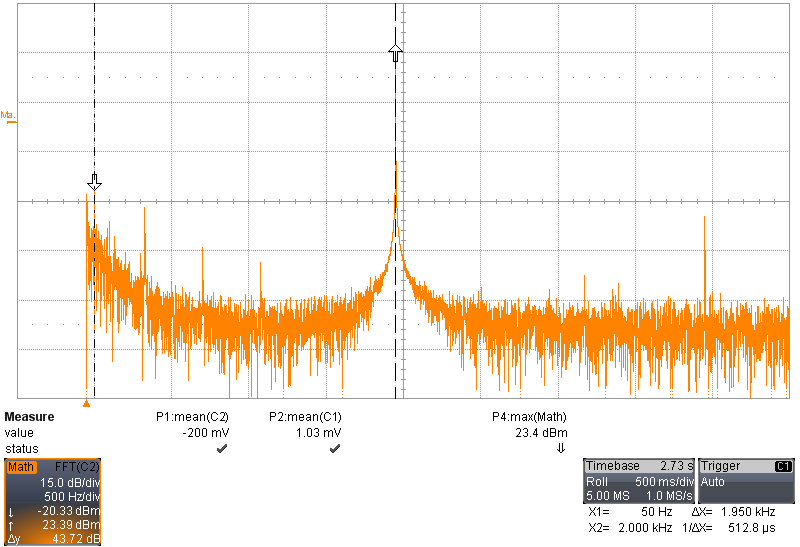
\includegraphics[scale=0.3]{figures/Results/Noisespectrum/sin2k-0_02v}}

  \caption[Kurze Abbildungsbeschreibung]{FFT-spectrum of integrated sine-wave at 2kHz}
\label{fig.noisefft}
\end{figure}

The spectral components of the lower frequencies in \ref{fig.noisefft} are relatively high when compared to the striking peak that can be attributed to the 2000 Hz fundamental frequency.
Furthermore, the amplitude of the lower frequencies is similar to the one of the first harmonic, i.e. 4000 Hz.
Judging from the results of this section, the two described non-idealities can not be neglected, the DC offset and the low frequency noise contribute significantly to the signal degradation and
most probably prevent the integrator from reducing the noise figure more considerably.


The following graph shows the influence or the air gap. 
\begin{figure}[htbp]
	\centering
	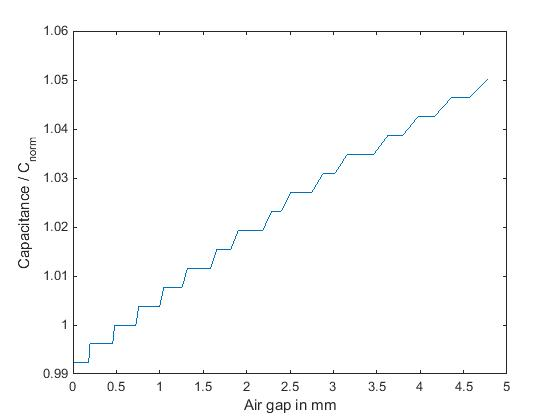
\includegraphics[width=0.5\textwidth]{figures/Results/airgap_height/airgap_graph.jpg}		
	\caption[Kurze Abbildungsbeschreibung]{Effect of a deviation of the air gap on the vacuum capacitance} \ref{fig.airgap}
	\label{fig.waveforms}
\end{figure}
 

The illustration of the height deviation proves that it is negligible and thus has no significant influence on the results. 
 \begin{figure}[htbp]
	\centering
	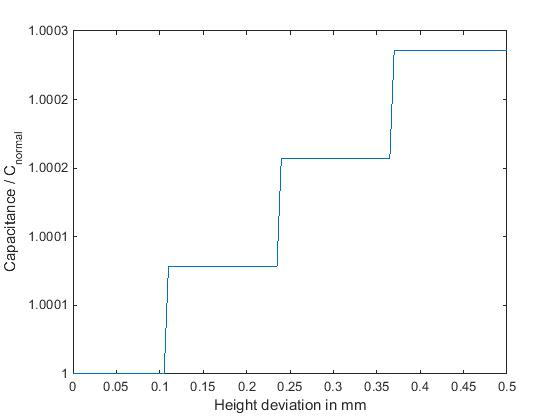
\includegraphics[width=0.5\textwidth]{figures/Results/airgap_height/Height_deviation.jpg}		
	\caption[Kurze Abbildungsbeschreibung]{Effect of a deviation in the height of the epoxid resin on the capacitance} \ref{fig.comsol_beispiel}
	\label{fig.waveforms}
\end{figure}